%-*-latex-*-
\sectionthree{Other types of asymptotic bounds}
\begin{python0}
from solutions import *; clear()
\end{python0}

In this section, all functions are functions of $n \in \N$.
I'll write $f$ instead of $f(n)$, etc.
I'll assume that all functions $f$ are asymptotically nonzero, i.e.,
there is some $N$ such that for all $n \geq N$, I will assume $f(n) \neq 0$.

Recall that $f = O(g)$ is
informally some kind of \lq\lq $\leq$" inequality:
a multiple of $g$ bounds $f$ from above asymptotically.
We also say that $f$ is \defone{asymptotically bounded above} by $g$.

It's also useful to have the concept of asymptotic \textit{lower} bound:

\begin{defn}
  We
  say $f$ is the \defone{big-$\Omega$} of $g$ and 
  write $f = \Omega(g)$ if
  there exist some $C > 0$ and some $N$ such that 
  for $n \geq N$,
  \[
  C|g(n)| \leq |f(n)|
  \]
  In other words a multiple of $g$ (asymptotically)
  bounds $f$ from \textit{below}.
  I will say that $f$ is \defone{asymptotically bounded below} by $g$.
\end{defn}

You can put the two definitions together and get this definition:

\begin{defn}
$f = \Theta(g)$ if $f = O(g)$ and $f = \Omega(g)$, i.e., 
there exist $C_1 > 0, N_1$ and $C_2 > 0, N_2$ such that
for $n \geq N_1$
\[
C_1|g(n)| \leq |f(n)|
\]
and for $n \geq N_2$,
\[
|f(n)| \leq C_2 |g(n)|
\]
If $f(n) = \Theta(g(n))$, I would say that
$f(n)$ has an \defone{asymptotic upper and lower bound} of $g(n)$.
Note that you don't need two cutoff points $N_1$ and $N_2$ for $n$
since if you
set $N = \max \{ N_1, N_2 \}$, then for $n \geq N$,
\[
C_1|g(n)| \leq |f(n)| \leq C_2 |g(n)|
\]
So the above definition is equivalent to this:
$f = \Theta(g)$ if there are constants $C_1 > 0, C_2 > 0$ and $N$ such that
for $n \geq N$,
\[
C_1|g(n)| \leq |f(n)| \leq C_2 |g(n)|
\]
\end{defn}

Informally, you want to think about $O$, $\Omega$, $\Theta$ roughly as:
\begin{align*}
f = O(g)      &\text{ \hspace{1cm} roughly \hspace{1cm} } f \text{\lq\lq$\leq$"} g \\
f = \Omega(g) &\text{ \hspace{1cm} roughly \hspace{1cm} } f \text{\lq\lq$\geq$"} g \\
f = \Theta(g) &\text{ \hspace{1cm} roughly \hspace{1cm} } f \text{\lq\lq$=$"} g
\end{align*}
Recall that you want your asymptotic upper and lower bound be as tight as
possible.
For instance it is true that
\[
n^2 + n + 1 = O(n^{100})
\]
But this is a tighter upper bound:
\[
n^2 + n + 1 = O(n^{2})
\]
This is the same for $\Omega$:
\[
n^2 + n + 1 = \Omega(n^1)
\]
So $O$ and $\Omega$ can be tight.

Here are some basic facts you should know.

\begin{prop}
  $f = O(g)$ iff $g = \Omega(f)$.
\end{prop}

\begin{prop}
  Let $f, g, h, f_i, g_i$ be functions of $n \in \N$ and $c \neq 0$ be a constant.
  \begin{myenum}
  \item
    \textsc{Reflexive:}
    \begin{align*}
    f &= O(f) \\
    f &= \Omega(f) \\
    f &= \Theta(f) 
    \end{align*}
  \item
    \textsc{Symmetric:}
    If $f,g$ are asyptotically nonzero, then
    \begin{align*}
    f = \Theta(g) \implies g = \Theta(f)
    \end{align*}  
  \item
    \textsc{Transitive:}
    \begin{align*}
    f = O(g) \text{, } g = O(h) &\implies f = O(h) \\
    f = \Omega(g) \text{, } g = \Omega(h) &\implies f = \Omega(h) \\
    f = \Theta(g) \text{, } g = \Theta(h) &\implies f = \Theta(h) \\
    \end{align*}
  \item
    \textsc{Antisymmetric:}
    \[
    f = O(g) \text{, } g = O(f) \implies f = \Theta(g)
    \]
  \end{myenum}
  \qed
\end{prop}

\begin{prop}
  \mbox{}
  \begin{myenum}
  \item
    \textsc{Summation:}
    \begin{align*}
    f_1 = O(g_1), \ f_2 = O(g_2) &\implies f_1 + f_2 = O \bigl( \max(|g_1|,|g_2|) \bigr) \\
    f_1 = \Omega(g_1), \ f_2 = \Omega(g_2) &\implies f_1 + f_2 = \Omega \bigl( \min(|g_1|,|g_2|) \bigr)
    \end{align*}
  \item
    \textsc{Product:}
    \begin{align*}
    f_1 = O(g_1), \ f_2 = O(g_2) &\implies f_1 f_2 = O(g_1 g_2) \\
    f_1 = \Omega(g_1), \ f_2 = \Omega(g_2) &\implies f_1 f_2 = \Omega(g_1 g_2) \\
    f_1 = \Theta(g_1), \ f_2 = \Theta(g_2) &\implies f_1 f_2 = \Theta(g_1 g_2) \\
    \end{align*}
  \end{myenum}
\end{prop}


\begin{cor}
    \begin{align*}
    f_1 = O(g), \ f_2 = O(g) &\implies f_1 + f_2 = O(g) \\
    f_1 = \Omega(g), \ f_2 = \Omega(g) &\implies f_1 + f_2 = \Omega(g) \\
    f_1 = \Theta(g), \ f_2 = \Theta(g) &\implies f_1 + f_2 = \Theta(g) 
    \end{align*}
\end{cor}

\begin{cor}
    \textsc{Constant cancellation:}
    \begin{align*}
      f = O(cg) \iff f = O(g)           &\text{ \,\,\, and \,\,\, } cf = O(g) \iff f = O(g) \\
      f = \Omega(cg) \iff f = \Omega(g) &\text{ \,\,\, and \,\,\, } cf = \Omega(g) \iff f = \Omega(g) \\
      f = \Theta(cg) \iff f = \Theta(g) &\text{ \,\,\, and \,\,\, } cf = \Theta(g) \iff f = \Theta(g)
    \end{align*}
\end{cor}

Now I mentioned earlier
\begin{align*}
n^2 + n + 1 &= O(n^2) \\
n^2 + n + 1 &= O(n^3) \\
n^2 + n + 1 &= O(n^{100}) \\
\end{align*}
There are times when I want to say $\lq\lq f$ is asymptotically bounded
above by $g$ but $g$ is \textit{not} a tight upper bound".
That's where  
the \lq\lq little" notations come in: 
the little-o and little-$\omega$.
($\omega$ is the lowercase of Greek $\Omega$.)

\begin{defn}
  Let $f,g$ be functions of $n$.
  \begin{myenum}
  \item
    $f = o(g)$\index{$o$@o}\tinysidebar{$o$}
    if for \textit{every} constant $C > 0$, there is some $N(C)$ such that
    for $n \geq N(C)$,
    \[
    |f(n)| \leq C |g(n)|
    \]
  \item
    $f = \omega(g)$\index{$\omega$@omega}\tinysidebar{$\omega$}
    if for \textit{every} constant $C > 0$, there is some $N(C)$ such that
    for $n \geq N(C)$,
    \[
    |f(n)| \leq C |g(n)|
    \]
  \end{myenum}
   Compare the definitions of little-o and big-O and then
   little-$\omega$ and big-$\Omega$ very carefully.
\end{defn}


What is the difference between little-o and big-O?
Just from the logic behind the two definitions, it's clear that
\[
f = o(g) \implies f = O(g)
\]
But what is the intuition behind the definition of little-o?
For now think of $C$ as a fixed number.
Then if $f = o(g)$, there is some $N(C)$ such that for
\[
n \geq N(C) \implies |f(n)| \leq C|g(n)|
\]
If I change $C$ to a larger number $C'$, I can use the same $N(C)$
for the above implication.
So no big deal.
But what if I replace $C$ by a smaller $C'$?
Then there is some $N(C')$ such that
\[
n \geq N(C') \implies |f(n)| \leq C'|g(n)|
\]
This basically says that no matter how small I \lq\lq shrink" $|g(n)|$
by a very tiny factor $C'$, the $C'|g(n)|$ still bound
$|f(n)|$.
In other words, if $f = o(g)$, then it means that
$g$ is an upper bound of $f$ in such a
way that no matter how I try to \lq\lq shrink $g$ by a constant
multiplier, $f$ can never go beyond $g$ (asymptotically).

Using a concrete example,
\[
100n^2 + n + 1 = O(n^2) \text{ and } 100n^2 + n + 1 = O(n^3)
\]
but
\[
100n^2 + n + 1 \neq o(n^2) \text{ and } 100n^2 + n + 1 = o(n^3)
\]
Therefore, informally, while you think of \lq\lq $f = O(g)$" as
roughly \lq\lq $f \leq g$, you think of \lq\lq $f = o(g)$"
as roughly \lq\lq $f < g$".

This is the same for little-$\omega$.
Informally, you want to think about $O$, $o$, $\Omega$, $\omega$, $\Theta$ roughly as:
\begin{align*}
f = O(g)      &\text{ \hspace{1cm} roughly \hspace{1cm} } f \text{\lq\lq$\leq$"} g \\
f = o(g)      &\text{ \hspace{1cm} roughly \hspace{1cm} } f \text{\lq\lq$<$"} g \\
f = \Omega(g) &\text{ \hspace{1cm} roughly \hspace{1cm} } f \text{\lq\lq$\geq$"} g \\
f = \omega(g) &\text{ \hspace{1cm} roughly \hspace{1cm} } f \text{\lq\lq$>$"} g \\
f = \Theta(g) &\text{ \hspace{1cm} roughly \hspace{1cm} } f \text{\lq\lq$=$"} g \\
\end{align*}

\begin{ex}
  Show that
  \begin{myenum}
  \item $1 \neq o(1)$ and $1 = o(n)$.
  \item $5n \neq o(12n)$ and $5n = o(2n^2)$.
  \item $100n^2 + n + 1 \neq o(n^2)$ and $100n^2 + n + 1 = o(n^3)$.
  \end{myenum}
\end{ex}


\begin{prop}
\mbox{}
\begin{myenum}
\item If $f = o(g)$, then $f = O(g)$. 
\item If $f = \omega(g)$, then $f = \Omega(g)$. 
\end{myenum}
\end{prop}



\begin{prop}
  \mbox{}
  \begin{myenum}
    \item
    \textsc{Transitivity:}
    \begin{align*}
      f = o(g) \text{, } g = o(h) &\implies f = o(h) \\
      f = \omega(g) \text{, } g = \omega(h) &\implies f = \omega(h)
    \end{align*}
  \item
    \textsc{Summation:}
    \begin{align*}
      f_1 = o(g_1), \ f_2 = o(g_2) &\implies f_1 + f_2 = o \bigl( \max(|g_1|,|g_2|) \bigr) \\
      f_1 = \omega(g_1), \ f_2 = \omega(g_2) &\implies f_1 + f_2 = \omega \bigl( \min(|g_1|,|g_2|) \bigr)
    \end{align*}
  \item
    \textsc{Product:}
    \begin{align*}
      f_1 = o(g_1), \ f_2 = o(g_2) &\implies f_1 f_2 = o(g_1 g_2) \\
      f_1 = \omega(g_1), \ f_2 = \omega(g_2) &\implies f_1 f_2 = \omega(g_1 g_2) 
    \end{align*}
  \end{myenum}
\end{prop}

\begin{cor}
    \begin{align*}
    f_1 = o(g), \ f_2 = o(g) &\implies f_1 + f_2 = o(g) \\
    f_1 = \omega(g), \ f_2 = \omega(g) &\implies f_1 + f_2 = \omega(g)
    \end{align*}
\end{cor}

\begin{cor}
    \textsc{Constant cancellation:}
    \begin{align*}
      f = o(cg) \iff f = o(g)           &\text{ \,\,\, and \,\,\, } cf = o(g) \iff f = o(g) \\
      f = \omega(cg) \iff f = \omega(g) &\text{ \,\,\, and \,\,\, } cf = \omega(g) \iff f = \omega(g)
    \end{align*}
\end{cor}


Besides \textit{inequality} types asymptotic bounds, there are also
\textit{limit} types asymptotic properties.
Here's one:

\begin{defn}
  $f$ and $g$ are \defone{asymptotically equivalent},
  and we write
  \[
  f(n) \sim g(n)
  \]
  if
  \[
  \lim_{n \rightarrow \infty} \frac{f(n)}{g(n)} = 1
  \]
\end{defn}

For instance
\[
\lim_{n \rightarrow \infty} \frac{n^2 + 1000\ln n}{n^2 + 10000n\sin(n)}
= 1
\]
This does \textit{not} mean that they actually meet, i.e., 
it does not mean that there is some $N$ such that 
for $n \geq N$, $f(n) = g(n)$.

Note that
\[
f \sim g
\]
is the not the same as
\[
f = \Theta(g)
\]
$f \sim g$ is clearly a lot tighter than $f = \Theta(g)$.
For instance
\[
\sin(n) = \Theta(1)
\]
But
\[
\sin(n) \not\sim (1)
\]

\begin{prop}
\mbox{}
\begin{myenum}
\item \textsc{Reflexive:} $f \sim f$
\item \textsc{Symmetric:} $f \sim g \implies g \sim f$
\item \textsc{Transitive:} $f \sim g, g \sim h \implies f \sim h$
\item \textsc{Summation:} $f_1 \sim g_1, f_2 \sim g_2
  \implies f_1 + f_2 \sim g_1 + g_2$
\item \textsc{Product:}
  $f_1 \sim f_2, g_1 \sim g_2
  \implies f_1 g_1 \sim f_2 g_2$
\item \textsc{Quotient:}
  If $f_2, g_2$ are asymptotically nonzero, then
  \[
  f_1 \sim g_1, f_2 \sim g_2 \implies f_1/f_2 \sim g_1/g_2
  \]
\end{myenum}
(a)-(c) says that asymptotic equivalence is an equivalence
relation.
\end{prop}

Recall that you can view big-$\Theta$ as a asymptotic rough version
of \lq\lq =".
Specifically $C_1|g(n)| \leq f(n) \leq C_2|g(n)|$ for large $n$.
There $C_1,C_2$ are some fixed constants.
Asymptotic equivalence is tighter than big-$\Theta$:

\begin{prop}
If $f \sim g$, then $f = \Theta(g)$. 
\end{prop}

Therefore if $\displaystyle\lim_{n \rightarrow \infty} \frac{f(n)}{g(n)}$ exists,
one can use $\displaystyle\lim_{n \rightarrow \infty} \frac{f(n)}{g(n)} = 0$ as the
definition of $f = o(g)$.
This is in fact done in some books.
But my definition is more general.

\begin{prop}
Assume $f, g$ are asymptotically $> 0$.
Suppose $\displaystyle \lim_{n \rightarrow \infty} \frac{f(n)}{g(n)}$ exists (including the case of $\infty$).
Let $L = \displaystyle \lim_{n \rightarrow \infty} \frac{f(n)}{g(n)}$.
Note that $L \in [0, \infty)$ or $L = \infty$.
For simplicity, I'll write, \lq\lq $L \in (0, \infty]$" as a shorthand for
\lq\lq $L \in (0, \infty)$ or $L = \infty$".
\begin{longtable}{rlcrl}
\textnormal{(a)} & $L \in [0, \infty) \iff f = O(g)$      & \hspace{1cm} & \textnormal{(d)} & $L = 0 \iff f = o(g)$  \\
\textnormal{(b)} & $L \in (0, \infty] \iff f = \Omega(g)$ & \hspace{1cm} & \textnormal{(e)} & $L = \infty \iff f = \omega(g)$ \\
\textnormal{(c)} & $L \in (0, \infty) \iff f = \Theta(g)$ & \hspace{1cm} & \textnormal{(f)} & $L = 1 \iff f \sim g$
\end{longtable}
\end{prop}
\proof
(d)
Let
\begin{myenum}
\item[1] $\lim_{n\rightarrow \infty} f(n)/g(n) = 0$ means:
  For all $\ep > 0$, there is some $N(\ep)$ such that
if $n \geq N(\ep)$, then $|f(n)/g(n) - 0| < \ep$.
The inequality is equivalent to $|f(n)| < \ep |g(n)|$.
\item[2] $f = o(g)$ means: For all $C > 0$, there is some $N(C)$ such that
$|f(n)| \leq C |g(n)|$.
\end{myenum}
Therefore I need to show (1)$\Longleftrightarrow$(2).

(1)$\Longrightarrow$(2):
Let $C > 0$. By (a), there is some $N(C)$ such that
for $n > N(C)$, $|f(n)| < C|g(n)|$ and hence $|f(n)| \leq C|g(n)|$.

(2)$\Longrightarrow$(1):
Let $\ep > 0$.
By (b), there is some $N(\ep/2)$ such that
for $n \geq N(\ep/2)$, $|f(n)| \leq (\ep/2)|g(n)|$, and hence
$|f(n)| \leq (\ep/2)|g(n)| < \ep |g(n)|$.
\qed

Therefore,
provided
$\displaystyle\lim_{n \rightarrow \infty} f(n)/g(n)$
exists, the above provides an alternative definition
for $O, \Omega, \Theta, o, \omega$.
For instance if $\displaystyle\lim_{n \rightarrow \infty} f(n)/g(n)$ exists,
then
\[
f = o(g) \iff \lim_{n \rightarrow} \frac{f(n)}{g(n)} = 0
\]


Therefore when $\displaystyle \lim_{n \rightarrow \infty} f(n)/g(n)$ exists, we can use Calculus to compute the
asymptotic relation between $f$ and $g$.
The following are some results that uses this technique.

\begin{prop}
  \mbox{}
  \begin{myenum}
  \item $\ln^a n = o(n^b)$ where $b/a > 0$ or $a = 0, b > 0$
  \item $n^b = o(c^n)$ where $c > 1$
  \end{myenum}
\end{prop}
\proof
(a)
Suppose $b/a > 0$.
\begin{align*}
  \lim_{n \rightarrow \infty} \frac{\ln^a n}{n^b}
  &= \lim_{n \rightarrow \infty} \left( \frac{\ln n}{n^{b/a}} \right)^a\\
  &= \lim_{n \rightarrow \infty} \left( \frac{1/n}{(b/a)n^{b/a - 1}} \right)^a & & \text{by l'H\^opital's rule}\\
  &= \lim_{n \rightarrow \infty} \left( \frac{1}{(b/a)n^{b/a}} \right)^a\\
  &= 0
\end{align*}
For the case $a = 0, b > 0$, $\ln^a n = 1$ and
$\displaystyle \lim_{n \rightarrow \infty} 1/n^b = 0$.
Hence in both cases $\ln^a n = o(n^b)$.

(b)
Suppose $b > 0$.
\begin{align*}
  \lim_{n \rightarrow \infty} \frac{n^b}{c^n}
  &= \lim_{n \rightarrow \infty} \left( \frac{n}{c^{n/b}} \right)^b\\
  &= \left( \lim_{n \rightarrow \infty} \frac{n}{c^{n/b}} \right)^b\\
  &= \left( \lim_{n \rightarrow \infty} \frac{1}{c^{n/b}(\ln c)(1/b)} \right)^b & & \text{by l'H\^opital's rule}\\
  &= \left( \frac{b}{\ln c} \cdot \lim_{n \rightarrow \infty} \frac{1}{c^{n/b}} \right)^b\\
  &= 0
\end{align*}
If $b \leq 0$,
$\displaystyle\lim_{n \rightarrow \infty} \frac{n^b}{c^n} = \lim_{n \rightarrow \infty} \frac{1}{n^{|b|}c^n} = 0$.
Hence in both cases $n^b = o(c^n)$.
\qed

\begin{prop}
  If $c < d$, then $c^n = o(d^n)$.
\end{prop}

The follow says that in any asymptotic relation, a function can be
replaced by another asymptotic equivalent function:

\begin{prop}
  Suppose $f_1 \sim f_2, g_1 \sim g_2$.
  \begin{myenum}
  \item $f_1 = O(g_1),  \implies f_2 = O(g_2)$
  \item $f_1 = \Omega(g_1),  \implies f_2 = \Omega(g_2)$
  \item $f_1 = \Theta(g_1),  \implies f_2 = \Theta(g_2)$
  \item $f_1 = o(g_1),  \implies f_2 = o(g_2)$
  \item $f_1 = \omega(g_1),  \implies f_2 = \omega(g_2)$
  \end{myenum}
\end{prop}

%\newpage
%\subsection*{Solutions}
%
\newpage
\section*{Solutions}
Solution to Exercise \ref{ex:dfa0}\labeltext{}{sol:dfa0}.

\tinysidebar{\debug{exercises/{dfa0/answer.tex}}}

    Solution not provided.
    

\newpage

Solution to Exercise \ref{ex:dfa1}\labeltext{}{sol:dfa1}.

\tinysidebar{\debug{exercises/{dfa1/answer.tex}}}
  The ID computation is
  \begin{align*}
    (q_0, aba)
    &\vdash (\delta(q_0, a), ba) = (q_0, ba) \\ 
    &\vdash (\delta(q_0, b), a) = (q_1, a) \\
    &\vdash (\delta(q_1, a), \ep) = (q_0, \ep)
  \end{align*}
  $q_0$ is not an accept state. Therefore $aba$ is not accepted.


\newpage

Solution to Exercise \ref{ex:dfa4}\labeltext{}{sol:dfa4}.

\tinysidebar{\debug{exercises/{dfa4/answer.tex}}}

    Solution not provided.
    

\newpage

Solution to Exercise \ref{ex:dfa5}\labeltext{}{sol:dfa5}.

\tinysidebar{\debug{exercises/{dfa5/answer.tex}}}

    Solution not provided.
    

\newpage

Solution to Exercise \ref{ex:implementing-a-single-dfa0}\labeltext{}{sol:implementing-a-single-dfa0}.

\tinysidebar{\debug{exercises/{implementing-a-single-dfa0/answer.tex}}}

    Solution not provided.
    

\newpage

Solution to Exercise \ref{ex:nfastatediag0}\labeltext{}{sol:nfastatediag0}.

\tinysidebar{\debug{exercises/{nfastatediag0/answer.tex}}}

    Solution not provided.
    

\newpage

Solution to Exercise \ref{ex:nfastatediag1}\labeltext{}{sol:nfastatediag1}.

\tinysidebar{\debug{exercises/{nfastatediag1/answer.tex}}}

    Solution not provided.
    

\newpage

Solution to Exercise \ref{ex:nfastatediag2}\labeltext{}{sol:nfastatediag2}.

\tinysidebar{\debug{exercises/{nfastatediag2/answer.tex}}}

    Solution not provided.
    

\newpage

Solution to Exercise \ref{ex:nfastatediag3}\labeltext{}{sol:nfastatediag3}.

\tinysidebar{\debug{exercises/{nfastatediag3/answer.tex}}}

    Solution not provided.
    

\newpage

Solution to Exercise \ref{ex:nfastatediag4}\labeltext{}{sol:nfastatediag4}.

\tinysidebar{\debug{exercises/{nfastatediag4/answer.tex}}}

    Solution not provided.
    

\newpage

Solution to Exercise \ref{ex:nfastatediag5}\labeltext{}{sol:nfastatediag5}.

\tinysidebar{\debug{exercises/{nfastatediag5/answer.tex}}}

    Solution not provided.
    

\newpage

Solution to Exercise \ref{ex:nfastatediag6}\labeltext{}{sol:nfastatediag6}.

\tinysidebar{\debug{exercises/{nfastatediag6/answer.tex}}}

    Solution not provided.
    

\newpage

Solution to Exercise \ref{ex:nfastatediag7}\labeltext{}{sol:nfastatediag7}.

\tinysidebar{\debug{exercises/{nfastatediag7/answer.tex}}}

    Solution not provided.
    

\newpage

Solution to Exercise \ref{ex:nfastatediag8}\labeltext{}{sol:nfastatediag8}.

\tinysidebar{\debug{exercises/{nfastatediag8/answer.tex}}}

    Solution not provided.
    

\newpage

Solution to Exercise \ref{ex:nfastatediag9}\labeltext{}{sol:nfastatediag9}.

\tinysidebar{\debug{exercises/{nfastatediag9/answer.tex}}}

    Solution not provided.
    

\newpage

Solution to Exercise \ref{ex:nfastatediag10}\labeltext{}{sol:nfastatediag10}.

\tinysidebar{\debug{exercises/{nfastatediag10/answer.tex}}}

    Solution not provided.
    

\newpage

Solution to Exercise \ref{ex:nfastatediag11}\labeltext{}{sol:nfastatediag11}.

\tinysidebar{\debug{exercises/{nfastatediag11/answer.tex}}}

    Solution not provided.
    

\newpage

Solution to Exercise \ref{ex:nfastatediag12}\labeltext{}{sol:nfastatediag12}.

\tinysidebar{\debug{exercises/{nfastatediag12/answer.tex}}}

    Solution not provided.
    

\newpage

Solution to Exercise \ref{ex:nfastatediag13}\labeltext{}{sol:nfastatediag13}.

\tinysidebar{\debug{exercises/{nfastatediag13/answer.tex}}}

    Solution not provided.
    

\newpage

Solution to Exercise \ref{ex:nfa0}\labeltext{}{sol:nfa0}.

\tinysidebar{\debug{exercises/{nfa0/answer.tex}}}
The formal definition of this NFA is $(\Sigma, Q, q_0, \delta, F)$ where
\begin{tightlist}
\li $\Sigma = \{a,b\}$
\li $Q = \{q_0\}$
\li $\delta$ is the function
\[
\delta : Q \times \Sigma_\epsilon \rightarrow P(Q)
\]
given by
\begin{align*}
  \delta(q_0, \epsilon) &= \{\} \\
  \delta(q_0, a) &= \{\} \\
  \delta(q_0, b) &= \{\} 
\end{align*}
\end{tightlist}


\newpage

Solution to Exercise \ref{ex:nfa1}\labeltext{}{sol:nfa1}.

\tinysidebar{\debug{exercises/{nfa1/answer.tex}}}

    Solution not provided.
    

\newpage

Solution to Exercise \ref{ex:nfa2}\labeltext{}{sol:nfa2}.

\tinysidebar{\debug{exercises/{nfa2/answer.tex}}}

    Solution not provided.
    

\newpage

Solution to Exercise \ref{ex:nfa3}\labeltext{}{sol:nfa3}.

\tinysidebar{\debug{exercises/{nfa3/answer.tex}}}

    Solution not provided.
    

\newpage

Solution to Exercise \ref{ex:nfa4}\labeltext{}{sol:nfa4}.

\tinysidebar{\debug{exercises/{nfa4/answer.tex}}}

    Solution not provided.
    

\newpage

Solution to Exercise \ref{ex:nfa5}\labeltext{}{sol:nfa5}.

\tinysidebar{\debug{exercises/{nfa5/answer.tex}}}

    Solution not provided.
    

\newpage

Solution to Exercise \ref{ex:dfa-as-powerful-as-nfa0}\labeltext{}{sol:dfa-as-powerful-as-nfa0}.

\tinysidebar{\debug{exercises/{dfa-as-powerful-as-nfa0/answer.tex}}}
Here's the solution.
Let $\delta$ denote the transition function of $N$.
Note that 
\begin{align*}
  \delta(q_0, \epsilon) = \{\} \\
  \delta(q_0, a) = \{\} \\
  \delta(q_0, b) = \{\} 
\end{align*}
First of all the states are labeled as all the subsets of $\{q_0\}$.


\begin{center}
\begin{tikzpicture}[>=triangle 60,shorten >=0.5pt,node distance=2cm,auto,initial text=, double distance=2pt]
\node[state] (A) at (  0,  0) {$\{q_0\}$};
\node[state] (B) at (  3,  0) {$\{\}$};

\path[->]

;
\end{tikzpicture}
\end{center}
    


The start state is the $\epsilon$-closure of $\{q_0\}$.
However in $N$, there are no $\epsilon$--transitions out of 
$q_0$.
So the $\epsilon$-closure of $\{q_0\}$ is in fact $\{q_0\}$, i.e.
$\overline{\{q_0\}} = \{q_0\}$
The $\DFA$ is now this:


\begin{longtable}{|r||r|r|r|r|r|}
\hline 
         & $w_1$ & $w_2$ & $w_3$ & $w_4$ & $\ldots$ \\ \hline \hline 
$M_1$    &       &       &       &       &          \\ \hline 
$M_2$    &       &       &       &       &          \\ \hline 
$M_3$    &       &       &       &       &          \\ \hline 
$M_4$    &       &       &       &       &          \\ \hline 
$\ldots$ &       &       &       &       &          \\ \hline 
\end{longtable}
        


Now I will compute the $a$--transition of the state $\{q_0\}$.
Let $\delta^\DFA$ denote the transition function of the $\DFA$
that we're building.
Then
\begin{align*}
\delta( \{q_0, a\} ) 
&= \overline{ \bigcup_{q \in \{q_0\}} \delta(q, a)} \\
&= \overline{ \delta(q_0, a) } \\
&= \overline{ \emptyset } \\
&= \emptyset
\end{align*}
The (incomplete) $\DFA$ now looks like this:


\begin{longtable}{|r||r|r|r|r|r|}
\hline 
         & $w_1$ & $w_2$ & $w_3$ & $w_4$ & $\ldots$ \\ \hline \hline 
$M_1$    & 0     & 0     & 1     & 0     & ...      \\ \hline 
$M_2$    & 1     & 0     & 1     & 1     & ...      \\ \hline 
$M_3$    & 0     & 1     & 1     & 1     & ...      \\ \hline 
$M_4$    & 1     & 0     & 1     & 1     & ...      \\ \hline 
$\ldots$ &       &       &       &       &          \\ \hline 
\end{longtable}
        


Using the same reasoning we have

\begin{center}
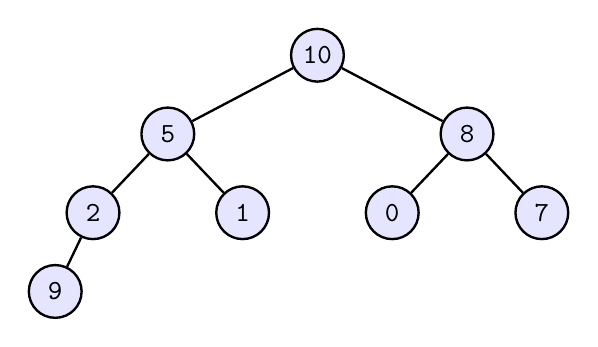
\begin{tikzpicture}

\fill[blue!10] (0.0, 0.0) circle (0.35);
\node [line width=0.03cm,black,minimum size=0.6699999999999999cm,draw,circle] at (0.0,0.0)(10){};\draw (0.0, 0.0) node[color=black] {\texttt{10}};
\fill[blue!10] (-1.9, -1.0) circle (0.35);
\node [line width=0.03cm,black,minimum size=0.6699999999999999cm,draw,circle] at (-1.9,-1.0)(5){};\draw (-1.9, -1.0) node[color=black] {\texttt{5}};
\fill[blue!10] (1.9, -1.0) circle (0.35);
\node [line width=0.03cm,black,minimum size=0.6699999999999999cm,draw,circle] at (1.9,-1.0)(8){};\draw (1.9, -1.0) node[color=black] {\texttt{8}};
\fill[blue!10] (-2.85, -2.0) circle (0.35);
\node [line width=0.03cm,black,minimum size=0.6699999999999999cm,draw,circle] at (-2.85,-2.0)(2){};\draw (-2.85, -2.0) node[color=black] {\texttt{2}};
\fill[blue!10] (-0.95, -2.0) circle (0.35);
\node [line width=0.03cm,black,minimum size=0.6699999999999999cm,draw,circle] at (-0.95,-2.0)(1){};\draw (-0.95, -2.0) node[color=black] {\texttt{1}};
\fill[blue!10] (0.95, -2.0) circle (0.35);
\node [line width=0.03cm,black,minimum size=0.6699999999999999cm,draw,circle] at (0.95,-2.0)(0){};\draw (0.95, -2.0) node[color=black] {\texttt{0}};
\fill[blue!10] (2.85, -2.0) circle (0.35);
\node [line width=0.03cm,black,minimum size=0.6699999999999999cm,draw,circle] at (2.85,-2.0)(7){};\draw (2.85, -2.0) node[color=black] {\texttt{7}};
\fill[blue!10] (-3.33, -3.0) circle (0.35);
\node [line width=0.03cm,black,minimum size=0.6699999999999999cm,draw,circle] at (-3.33,-3.0)(9){};\draw (-3.33, -3.0) node[color=black] {\texttt{9}};\draw[line width=0.03cm,black] (10) to  (5);
\draw[line width=0.03cm,black] (10) to  (8);
\draw[line width=0.03cm,black] (5) to  (2);
\draw[line width=0.03cm,black] (5) to  (1);
\draw[line width=0.03cm,black] (8) to  (0);
\draw[line width=0.03cm,black] (8) to  (7);
\draw[line width=0.03cm,black] (2) to  (9);
\end{tikzpicture}

\end{center}



It's easy to see that in the DFA, the $a$--
and $b$--transitions from the state $\{\}$ goes back to itself.
Therefore the completed DFA is this:


\begin{center}
\begin{tikzpicture}[>=triangle 60,shorten >=0.5pt,node distance=2cm,auto,initial text=, double distance=2pt]
\node[state,initial] (A) at (  0,  0) {$\{q_0\}$};
\node[state] (B) at (  3,  0) {$\{\}$};

\path[->]
(A) edge [bend left=0,pos=0.5,above] node {$a,b$} (B)
(B) edge [loop above] node {$a,b$} ()

;
\end{tikzpicture}
\end{center}
    



\newpage

Solution to Exercise \ref{ex:dfa-as-powerful-as-nfa1}\labeltext{}{sol:dfa-as-powerful-as-nfa1}.

\tinysidebar{\debug{exercises/{dfa-as-powerful-as-nfa1/answer.tex}}}

    Solution not provided.
    

\newpage

Solution to Exercise \ref{ex:dfa-as-powerful-as-nfa2}\labeltext{}{sol:dfa-as-powerful-as-nfa2}.

\tinysidebar{\debug{exercises/{dfa-as-powerful-as-nfa2/answer.tex}}}

    Solution not provided.
    

\newpage

Solution to Exercise \ref{ex:dfa-as-powerful-as-nfa3}\labeltext{}{sol:dfa-as-powerful-as-nfa3}.

\tinysidebar{\debug{exercises/{dfa-as-powerful-as-nfa3/answer.tex}}}

    Solution not provided.
    

\newpage

Solution to Exercise \ref{ex:dfa-as-powerful-as-nfa4}\labeltext{}{sol:dfa-as-powerful-as-nfa4}.

\tinysidebar{\debug{exercises/{dfa-as-powerful-as-nfa4/answer.tex}}}

    Solution not provided.
    

\newpage

Solution to Exercise \ref{ex:closure0}\labeltext{}{sol:closure0}.

\tinysidebar{\debug{exercises/{closure0/answer.tex}}}

    Solution not provided.
    

\newpage

Solution to Exercise \ref{ex:closure1}\labeltext{}{sol:closure1}.

\tinysidebar{\debug{exercises/{closure1/answer.tex}}}

    Solution not provided.
    

\newpage

Solution to Exercise \ref{ex:closure2}\labeltext{}{sol:closure2}.

\tinysidebar{\debug{exercises/{closure2/answer.tex}}}

    Solution not provided.
    

\newpage

Solution to Exercise \ref{ex:closure3}\labeltext{}{sol:closure3}.

\tinysidebar{\debug{exercises/{closure3/answer.tex}}}

    Solution not provided.
    

\newpage

Solution to Exercise \ref{ex:closure4}\labeltext{}{sol:closure4}.

\tinysidebar{\debug{exercises/{closure4/answer.tex}}}

    Solution not provided.
    

\newpage

Solution to Exercise \ref{ex:closure5}\labeltext{}{sol:closure5}.

\tinysidebar{\debug{exercises/{closure5/answer.tex}}}

    Solution not provided.
    

\newpage

Solution to Exercise \ref{ex:closure6}\labeltext{}{sol:closure6}.

\tinysidebar{\debug{exercises/{closure6/answer.tex}}}

    Solution not provided.
    

\newpage

Solution to Exercise \ref{ex:closure7}\labeltext{}{sol:closure7}.

\tinysidebar{\debug{exercises/{closure7/answer.tex}}}

    Solution not provided.
    

\newpage

Solution to Exercise \ref{ex:closure8}\labeltext{}{sol:closure8}.

\tinysidebar{\debug{exercises/{closure8/answer.tex}}}

    Solution not provided.
    

\newpage

Solution to Exercise \ref{ex:closure9}\labeltext{}{sol:closure9}.

\tinysidebar{\debug{exercises/{closure9/answer.tex}}}

    Solution not provided.
    

\newpage

Solution to Exercise \ref{ex:closure10}\labeltext{}{sol:closure10}.

\tinysidebar{\debug{exercises/{closure10/answer.tex}}}

    Solution not provided.
    

\newpage

Solution to Exercise \ref{ex:closure11}\labeltext{}{sol:closure11}.

\tinysidebar{\debug{exercises/{closure11/answer.tex}}}

    Solution not provided.
    

\newpage

Solution to Exercise \ref{ex:closure12}\labeltext{}{sol:closure12}.

\tinysidebar{\debug{exercises/{closure12/answer.tex}}}

    Solution not provided.
    

